% !TeX spellcheck = en_GB
\documentclass[main.tex]{subfiles}

\begin{document}
\chapter{Result Details}
\lhead{Appendix}

\section{Experiment: No Weight Fixing in Pretraining}
\label{sec:nofix}
This experiment was conducted as an ablation study on the locking of da-BERT weights.
All hyperparameters are the same as in the baseline experiment, described in Section \ref{subsec:baseline}, with the exception that the weights from da-BERT were unlocked for the entire pretraining.

\begin{table}[H]
    \centering
    \small
    \begin{tabular}{l|l|cccccc}
        Model                           & Top $k$ accuracy [\pro]  & $k=1$  & $k=3$ & $k=5$ & $k=10$ & $k=25$ & $k=50$\\\hline
        \multirow{2}{*}{Baseline}       & Masked words             & 24.4  & 31.2 & 34.6 & 39.9  & 47.7  & 53.7 \\
        & Masked entities          & 37.7  & 48.7 & 53.6 & 60.3  & 68.7  & 75.0
    \end{tabular}
    \caption{
        The top $k$ accuracy of the model with no parameter fixing in the 50'th and last epoch.
    }
    \label{tab:nofix-mlm}
\end{table}\noindent

\begin{figure}[H]
    \centering
    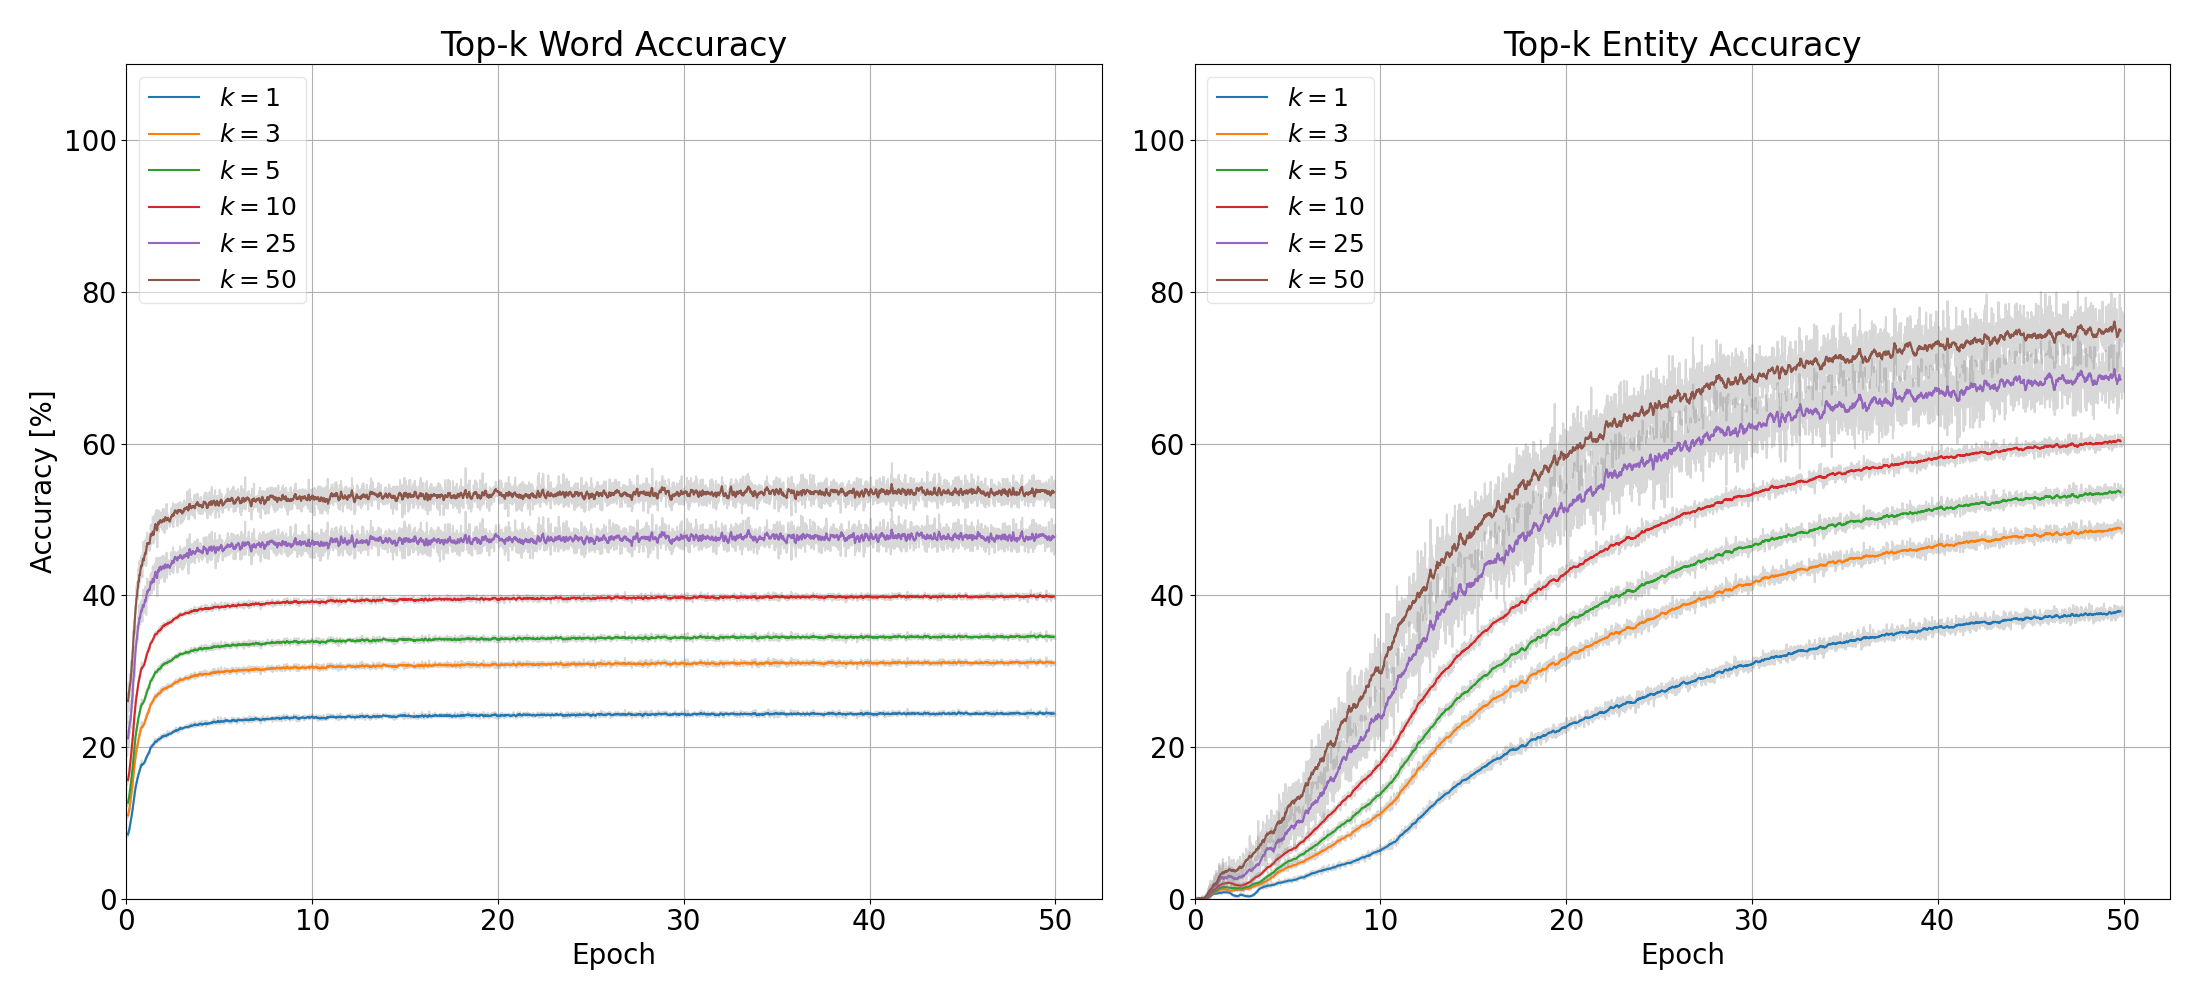
\includegraphics[width=\textwidth]{no-fix-acc}
    \caption{Development of masked language and masked entities when all weights are unlocked for the entire pretraining.}
\end{figure}\noindent

%2021-06-28 09:58:10.885    INFO                      precision    recall  f1-score   support
%
%LOC     0.8529    0.9062    0.8788        96
%MISC     0.7358    0.6446    0.6872       121
%ORG     0.8168    0.6646    0.7329       161
%PER     0.9489    0.9278    0.9382       180
%
%micro avg     0.8524    0.7867    0.8183       558
%macro avg     0.8386    0.7858    0.8093       558
%weighted avg     0.8481    0.7867    0.8143       558
\begin{table}[H]
    \centering
    \small
    \begin{tabular}{l|ccccc|c|c}
        \multirow{2}{*}{Model}  & \multicolumn{5}{c|}{F1 [\pro]} & Precision [\pro]               & Recall [\pro]               \\
        & Avg. & LOC & PER & ORG & MISC      & Avg.                           & Avg.                         \\ \hline
        No weight fixing & 81.8 & 87.9 & 93.8 & 73.3 & 68.7 & 85.2 & 78.7
    \end{tabular}
    \caption{The fine-tuning results of the weight unlocking pretraining experiment.}
    \label{tab:nofix}
\end{table}\noindent

\section{Fine-tuning Hyperparameter Search Results}
\label{sec:hyperres}

\begin{table}[H]
    \footnotesize
    \begin{tabular}{lllll|rrr}
        Batch size & Learning rate & Weight decay & Dropout & Loss weight & F1 [\%]    &  Precision & Recall\\\hline
        8& 1\ctp{-5}& 0.01& 0.025& Yes       & 73.06 &  62.82 &  87.29\\
        8& 1\ctp{-5}& 0.01& 0.025& No        & 73.53 &  62.87 &  88.54\\
        8& 1\ctp{-5}& 0.01& 0.1& Yes         & 73.52 &  63.17 &  87.92\\
        8& 1\ctp{-5}& 0.01& 0.1& No          & 71.39 &  60.00 &  88.12\\
        8& 1\ctp{-5}& 0.05& 0.025& Yes       & 72.87 &  62.54 &  87.29\\
        8& 1\ctp{-5}& 0.05& 0.025& No        & 67.77 &  56.07 &  85.62\\
        8& 1\ctp{-5}& 0.05& 0.1& Yes         & 71.44 &  60.46 &  87.29\\
        8& 1\ctp{-5}& 0.05& 0.1& No          & 71.91 &  61.45 &  86.67\\
        8& 5\ctp{-5}& 0.01& 0.025& Yes       & 83.08 &  77.14 &  90.00\\
        8& 5\ctp{-5}& 0.01& 0.025& No        & \textbf{85.35} &  \textbf{80.82} &  90.42\\
        8& 5\ctp{-5}& 0.01& 0.1& Yes         & 84.96 &  80.45 &  90.00\\
        8& 5\ctp{-5}& 0.01& 0.1& No          & 31.53 &  19.86 &  76.46\\
        8& 5\ctp{-5}& 0.05& 0.025& Yes       & 84.00 &  79.41 &  89.17\\
        8& 5\ctp{-5}& 0.05& 0.025& No        & 84.24 &  77.78 &  \textbf{91.88}\\
        8& 5\ctp{-5}& 0.05& 0.1& Yes         & 84.65 &  79.74 &  90.21\\
        8& 5\ctp{-5}& 0.05& 0.1& No          & \textbf{85.35} &  \textbf{80.82} &  90.42\\
        16& 1\ctp{-5}& 0.01& 0.025& Yes      & 65.29 &  52.76 &  85.62\\
        16& 1\ctp{-5}& 0.01& 0.025& No       & 63.91 &  51.12 &  85.21\\
        16& 1\ctp{-5}& 0.01& 0.1& Yes        & 63.33 &  50.24 &  85.62\\
        16& 1\ctp{-5}& 0.01& 0.1& No         & 62.57 &  49.57 &  84.79\\
        16& 1\ctp{-5}& 0.05& 0.025& Yes      & 63.73 &  50.61 &  86.04\\
        16& 1\ctp{-5}& 0.05& 0.025& No       & 63.63 &  50.55 &  85.83\\
        16& 1\ctp{-5}& 0.05& 0.1& Yes        & 64.13 &  51.11 &  86.04\\
        16& 1\ctp{-5}& 0.05& 0.1& No         & 63.06 &  49.70 &  86.25\\
        16& 5\ctp{-5}& 0.01& 0.025& Yes      & 84.83 &  79.10 &  91.46\\
        16& 5\ctp{-5}& 0.01& 0.025& No       & 83.72 &  78.26 &  90.00\\
        16& 5\ctp{-5}& 0.01& 0.1& Yes        & 82.66 &  76.88 &  89.38\\
        16& 5\ctp{-5}& 0.01& 0.1& No         & 29.21 &  18.08 &  76.04\\
        16& 5\ctp{-5}& 0.05& 0.025& Yes      & 83.67 &  77.25 &  91.25\\
        16& 5\ctp{-5}& 0.05& 0.025& No       & 83.60 &  76.70 &  \textbf{91.88}\\
        16& 5\ctp{-5}& 0.05& 0.1& Yes        & 83.29 &  76.90 &  90.83\\
        16& 5\ctp{-5}& 0.05& 0.1& No         & 82.94 &  76.45 &  90.62
    \end{tabular}
    \caption{
        The results of hyperparameter search with micro average percentages for the metrics reported on the DaNE test set.
    }
    \label{tab:hyperres}
\end{table}
\chapter{Additional Figures}
\section{Dimensionality Reduction}
\label{sec:dimredu}

\begin{figure}[H]
    \centering
        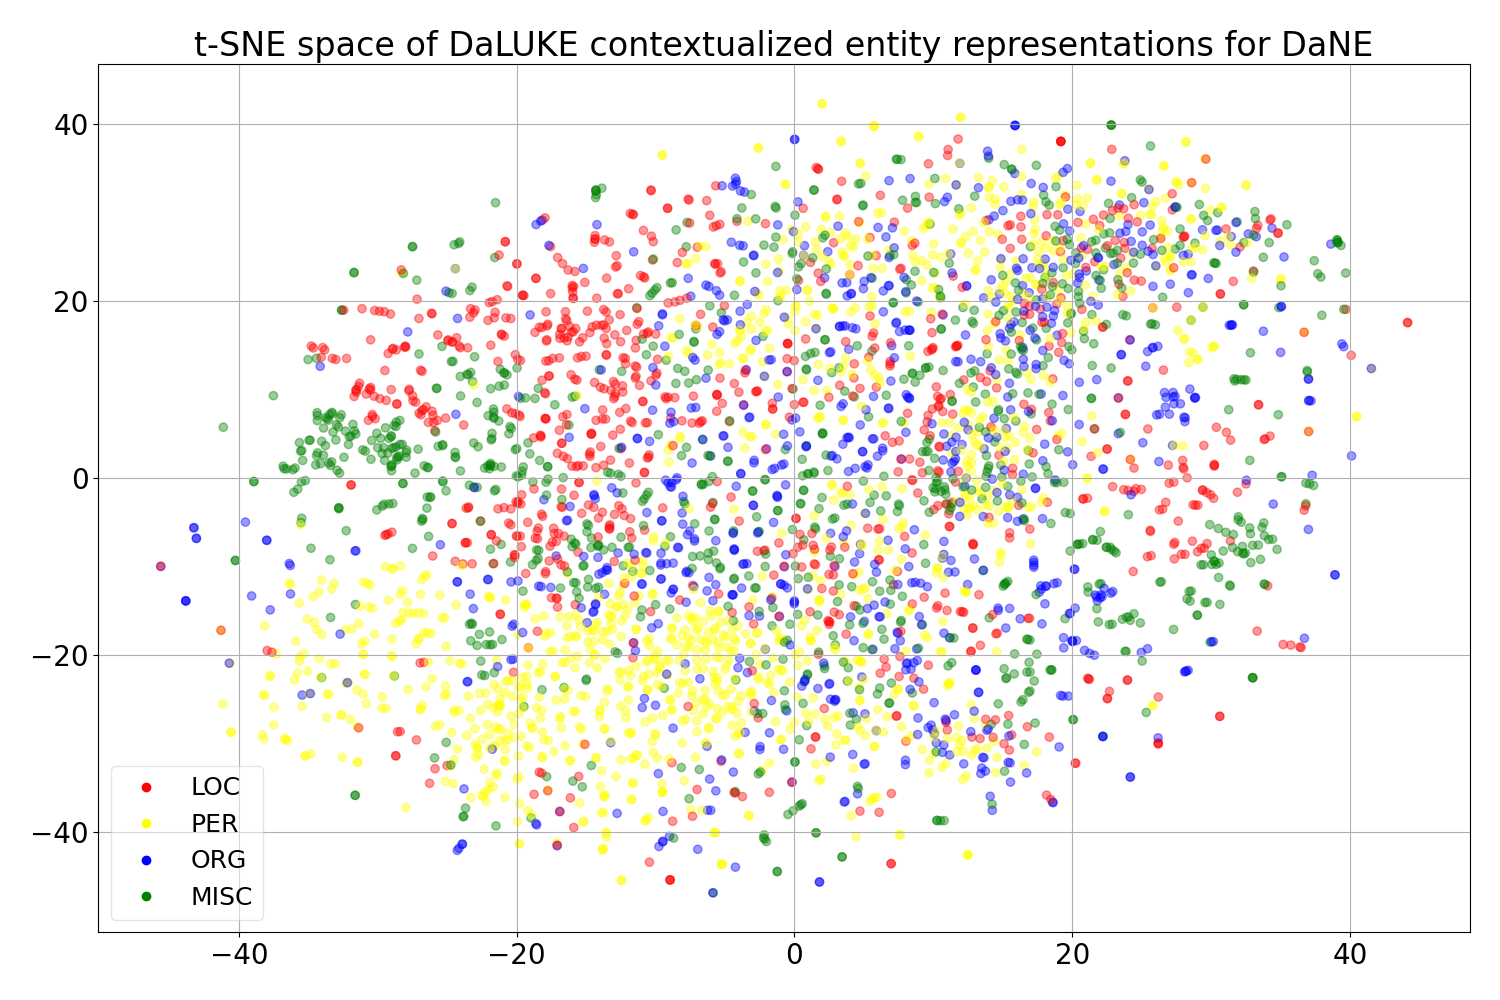
\includegraphics[width=0.8\linewidth]{full-geo/tsne}
    \caption{
        $t$-SNE performed on a 100K random subset of the full$\sim$ 1M possible entity spans in the training set of DaNE.
    }
    \label{fig:full-tsne}
\end{figure}\noindent

\begin{figure}[H]
    \centering
        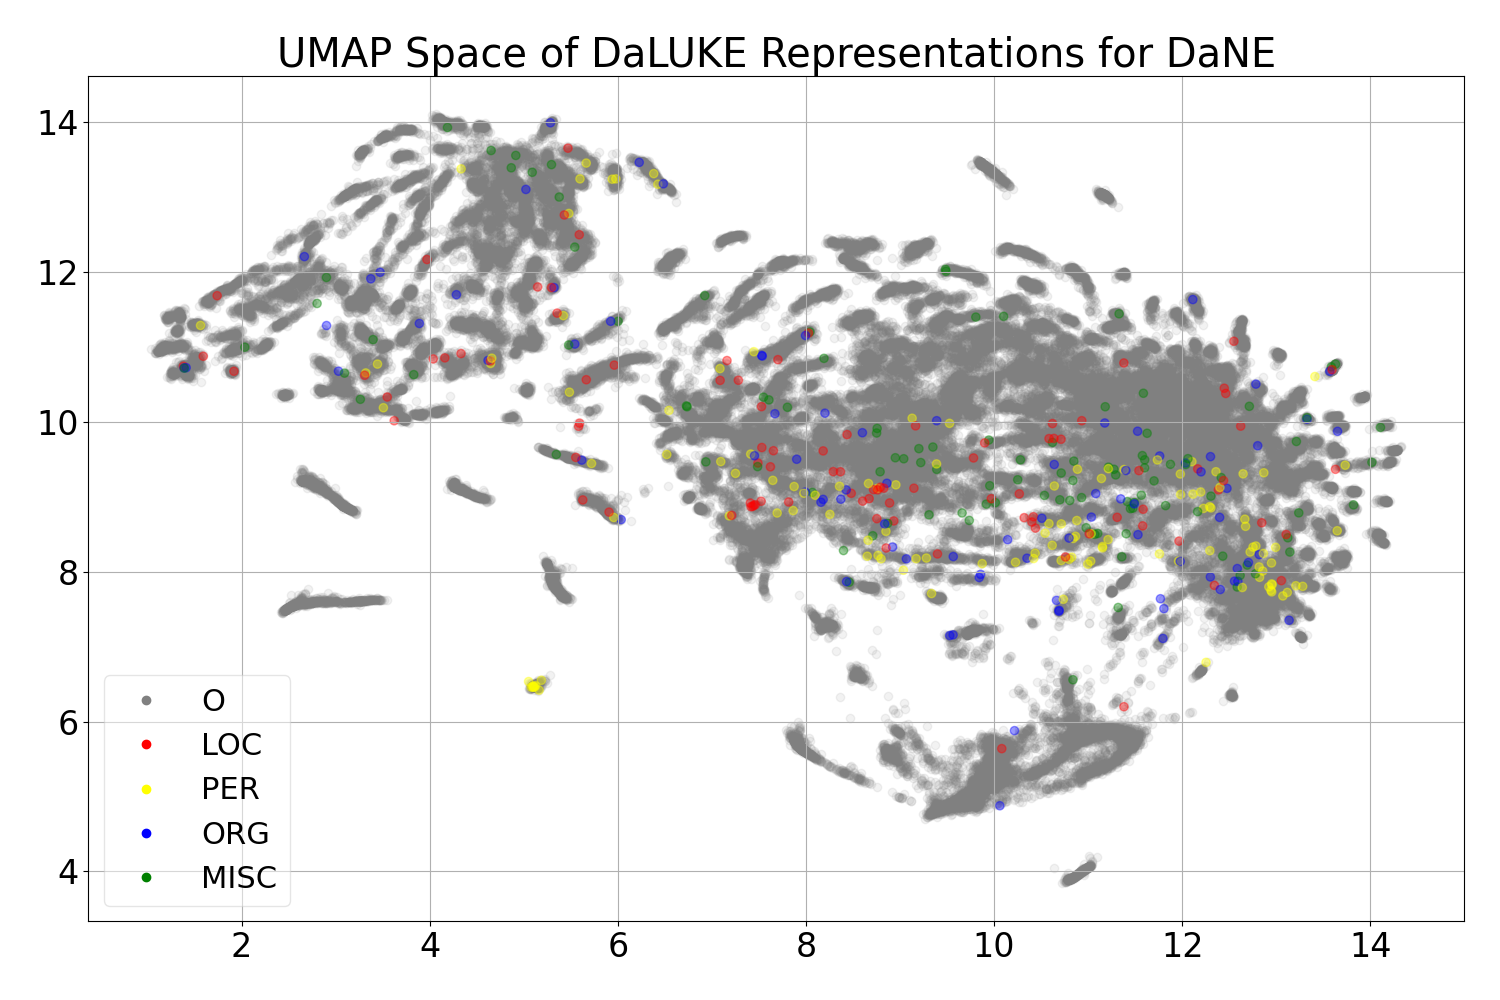
\includegraphics[width=0.8\linewidth]{full-geo/umap}
    \caption{
        UMAP performed on a 100K random subset of the full $\sim$ 1M possible entity spans in the DaNE training set.
    }
    \label{fig:full-umap}
\end{figure}\noindent

\begin{figure}[H]
    \centering
        \includegraphics[width=.8\linewidth]{full-geo/variance_explained}
    \caption{
        Variance explained by principal components found by PCA on full DaNE training dataset.
    }
    \label{fig:full-varex}
\end{figure}\noindent

\begin{figure}[H]
    \centering
        \includegraphics[width=.8\linewidth]{pos-geo/variance_explained}
    \caption{
        Variance explained by principal components found by PCA on the dataset including positive labels.
    }
    \label{fig:pos-varex}
\end{figure}\noindent

\end{document}
